\section{Resultate und Diskussion}\label{sec:diskussion}
Die theoretischen Werte und ihre gemessen Pendants sind in Tabelle \ref{tab:final} gezeigt. Die gemessen Werte stimmen relativ gut, jedoch gibt es einige Ausreisser. Das Loch mit $150\mu m$ Durchmesser ist mit grosser Wahrscheinlichkeit falsch beschriftet. Die Messung des Doppelspalten hat einen Fehler der grösser ist als bei den andern Messungen. Auf die Gründe wird in entsprechenden Kapitel eingegangen. Für die anderen wird ein visueller Vergleich dargestellt.

\begin{table}[H]
	\centering
	\begin{tabular}{ccc}
		Spalt $50\mu m$:		&  $49e-6$  	&  $\pm7e-7$\\
		Spalt $200\mu m$:		&  $196e-6$		&  $\pm6e-6$\\
		Antispalt $0.33mm$: 	&  $331e-6$		&  $\pm3e-6$\\
		Antispalt $0.124mm$:	&  $124e-6$		&  $\pm1e-6$\\
		Loch $150\mu m$: 		&  $69e-6$		&  $\pm4e-6$\\
		Loch $100\mu m$: 		&  $96e-6$		&  $\pm4e-6$\\
		Gitter $70\mu m$:  		&  $70e-6$		&  $\pm5e-6$\\
		Doppelspalt $40\mu m$: 	&  $616e-7$		&  $\pm5e-7$\\
	\end{tabular}
	\caption{Errechnete Endwerte}
	\label{tab:final}
\end{table}

\begin{figure}[H]
	\centering
	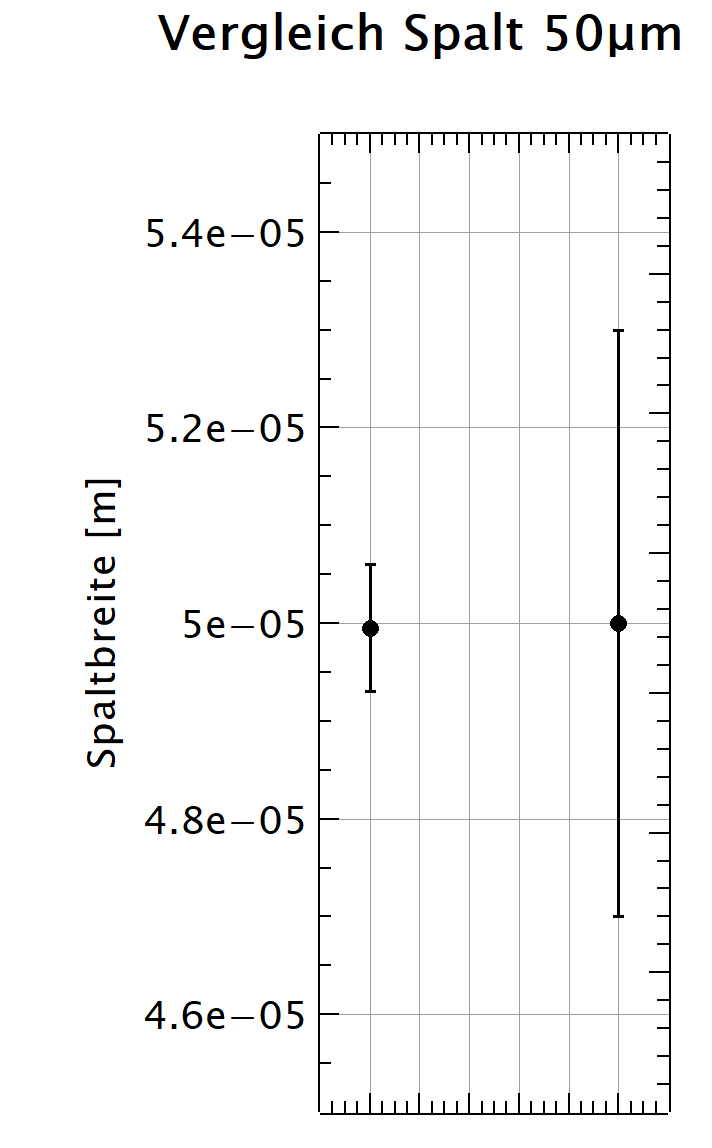
\includegraphics[width=0.4\textwidth]{data/dis_sp_50.png}
	\caption{Vergleich der gemessenen Werten mit den Theoretischen des $50\mu m$ Spalts}
	\label{fig:dis_spalt_50}
\end{figure}
\begin{figure}[H]
	\centering
	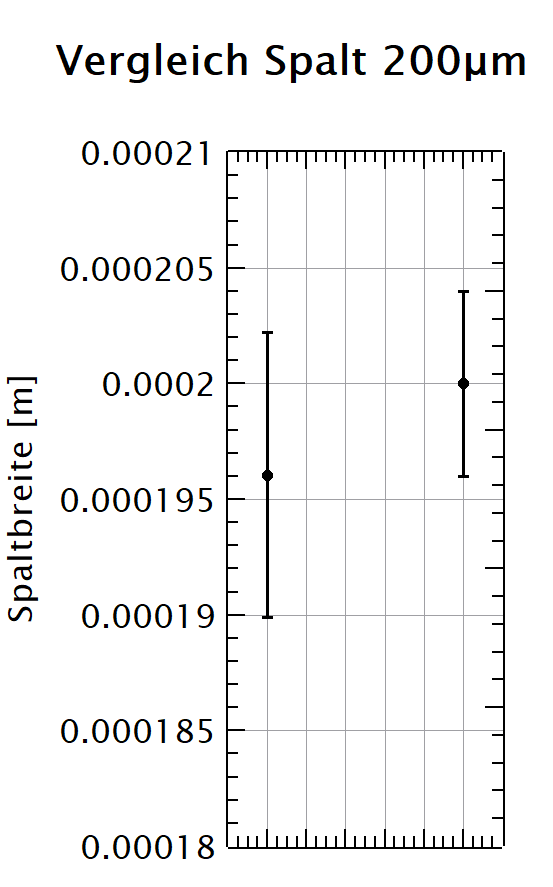
\includegraphics[width=0.4\textwidth]{data/dis_sp_200.png}
	\caption{Vergleich der gemessenen Werten mit den Theoretischen des $200\mu m$ Spalts}
	\label{fig:dis_spalt_200}
\end{figure}
\begin{figure}[H]
	\centering
	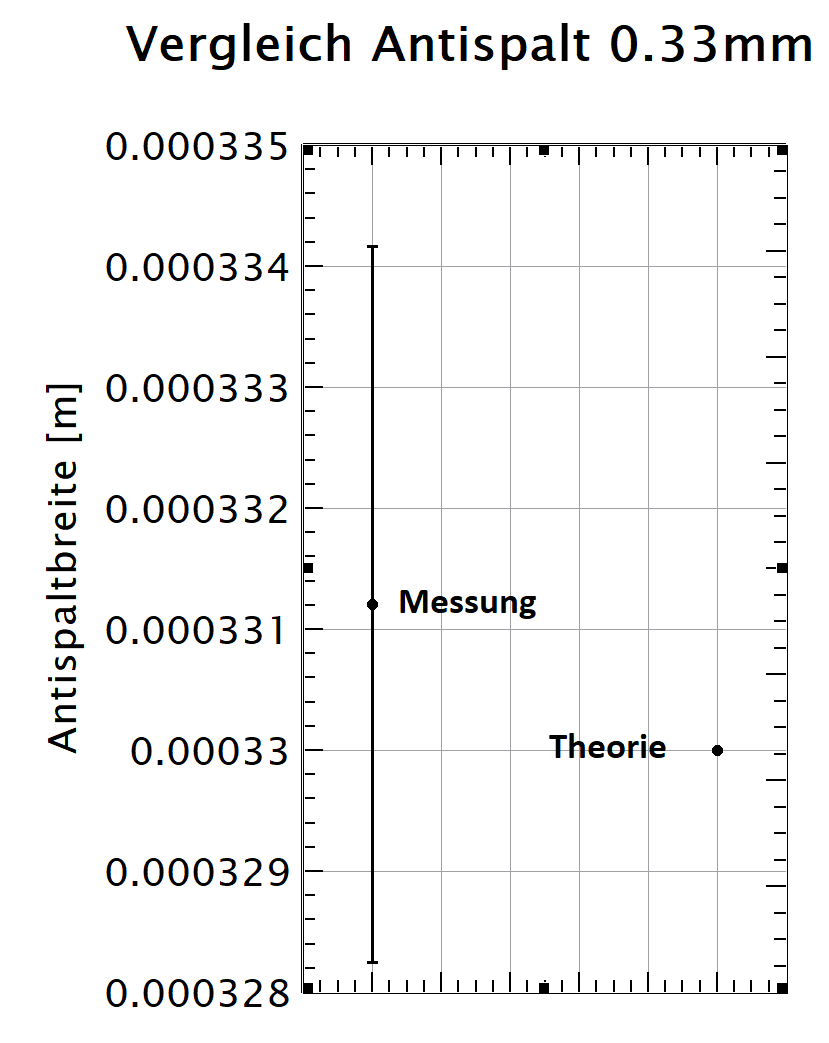
\includegraphics[width=0.4\textwidth]{data/dis_asp_33.png}
	\caption{Vergleich der gemessenen Werten mit den Theoretischen des $0.33mm$ Antispalts}
	\label{fig:dis_aspalt_33}
\end{figure}
\begin{figure}[H]
	\centering
	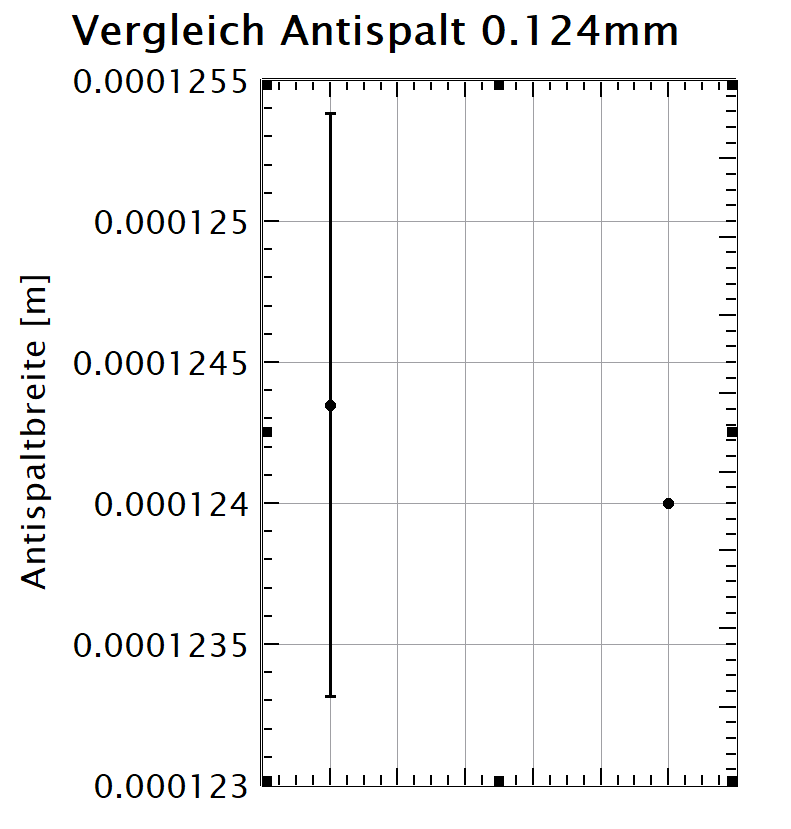
\includegraphics[width=0.4\textwidth]{data/dis_asp_12.png}
	\caption{Vergleich der gemessenen Werten mit den Theoretischen des $0.124mm$ Antispalts}
	\label{fig:dis_aspalt_12}
\end{figure}
\begin{figure}[H]
	\centering
	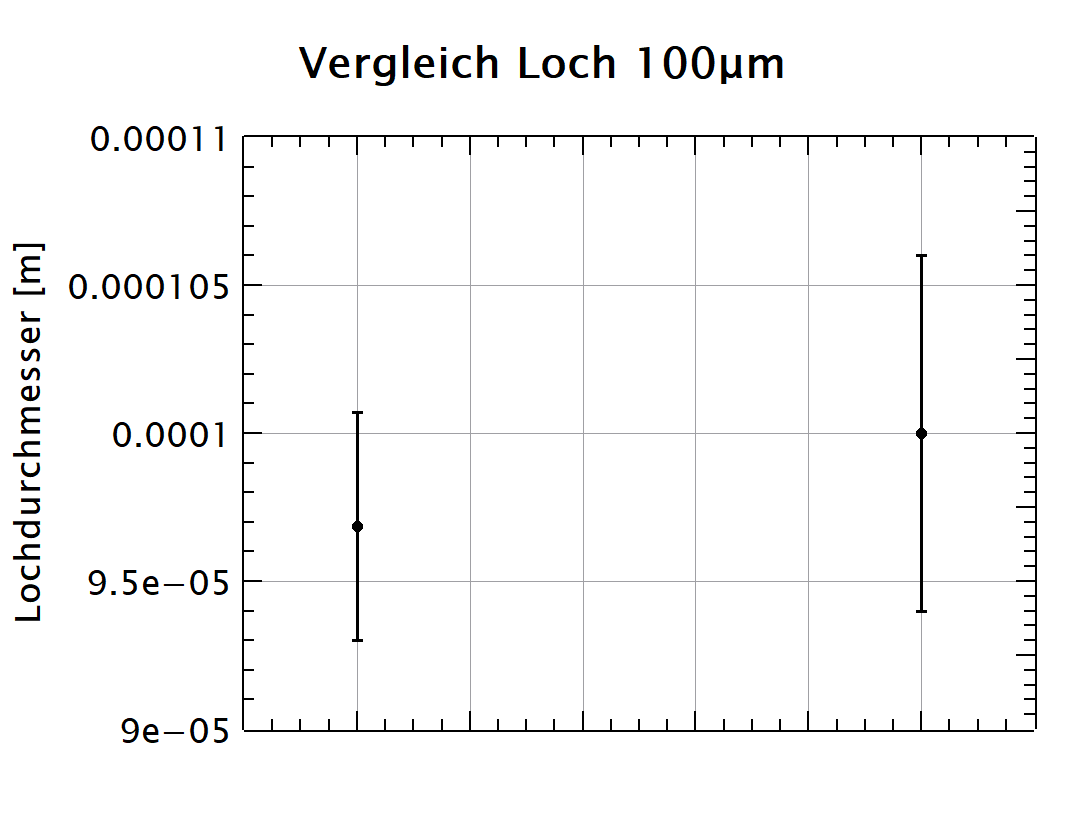
\includegraphics[width=0.4\textwidth]{data/dis_loch_100.png}
	\caption{Vergleich der gemessenen Werten mit den Theoretischen des $100\mu m$ Loch}
	\label{fig:dis_loch_100}
\end{figure}
\begin{figure}[H]
	\centering
	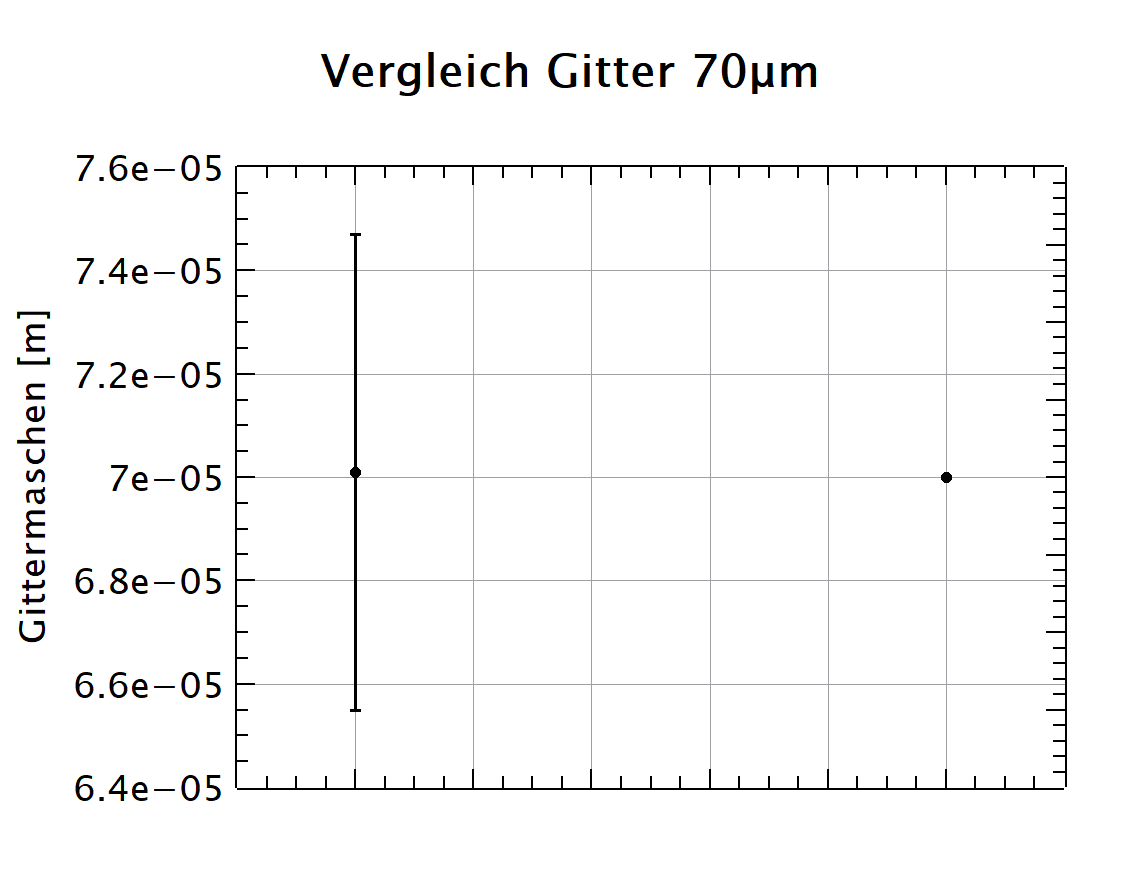
\includegraphics[width=0.4\textwidth]{data/dis_gitter.png}
	\caption{Vergleich der gemessenen Werten mit den Theoretischen des $70\mu m$ Gitter}
	\label{fig:dis_gitter}
\end{figure}

\subsection*{Loch $150\mu m$}
Zu sehen ist im visuellen Vergleich \ref{fig:dis_loch_150}, dass der theoretisch Wert weit entfernt der Messung liegt. Auch liegt die Messung nicht innerhalb der Toleranz  der Messprobe. Dies legt nahe, dass entweder die Auswertung, die Messung oder die Probe fehlerhaft sind.
\begin{figure}[H]
	\centering
	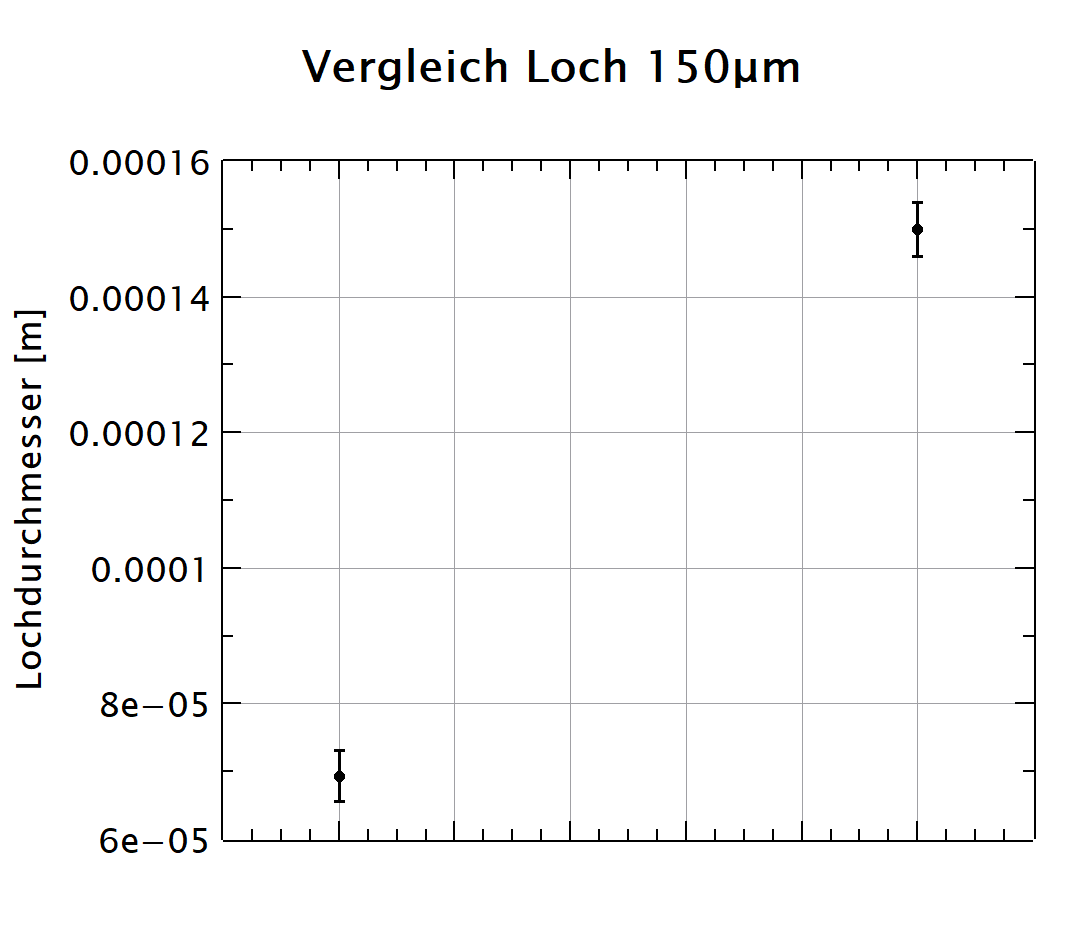
\includegraphics[width=0.4\textwidth]{data/dis_loch_150.png}
	\caption{Vergleich der gemessenen Werten mit den Theoretischen des $150\mu m$ Loch}
	\label{fig:dis_loch_150}
\end{figure}
Um einen Fehler bei der Auswertung auszuschliessen wurden die Messwert mit einer alternativen Variante ausgewertet. Mit QtiPlot ist Abbildung \ref{fig:dis_loch_fail} entstanden. Mit ihr ist gut zu sehen, dass die alternative Variante die selben Resultate liefert. Dadurch kann man sagen, dass wahrscheinlich kein Auswertungsfehler vorliegt.
\begin{figure}[H]
	\centering
	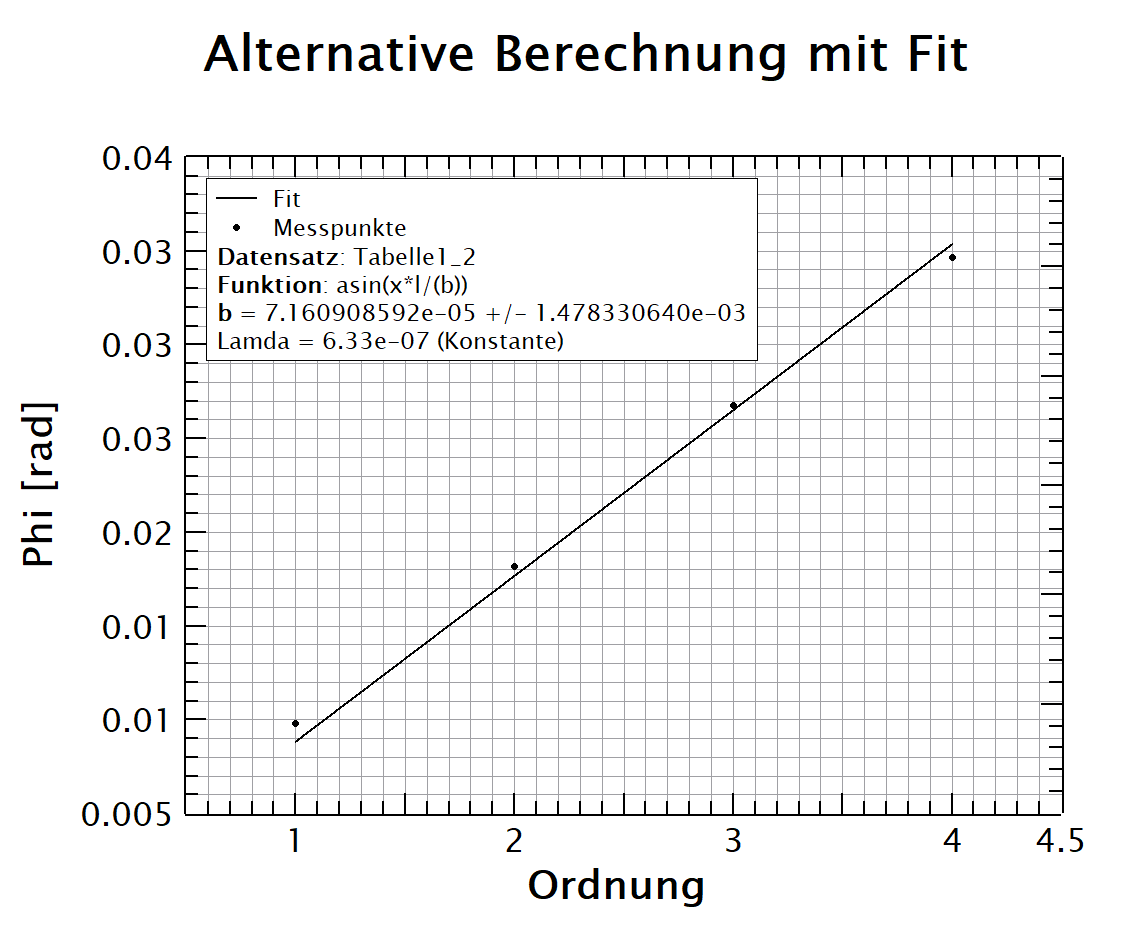
\includegraphics[width=0.4\textwidth]{data/fit_felerhaftes_loch.png}
	\caption{Überprüfung des gemessenen Lochs mit Alternativer Messmethode}
	\label{fig:dis_loch_fail}
\end{figure}

Des Weiteren kann ein Messungsfehler ausgeschlossen werden, weil alle andern Messungen stimmen. Somit bleibt nur noch die falsche Beschriftung der Messprobe übrig. Wir vermuten dies ist die Fehlerquelle.

\subsection*{Doppelspalt $40\mu m$}
Wichtig ist das Mann Brot einfrieren kann. Dadurch wird die Haltbarkeit massiv erhöht. Dieser Effekt lässt sich erhöhen, wenn das Brot nach Norden ausgerichtet ist. Die Messung des Doppelspalt stellte eine Schwierigkeit dar. Durch die schwachen Minimas auf der Blende, war die Messung schwierig. Dadurch sind die grossen Fehler entstanden.
\begin{figure}[H]
	\centering
	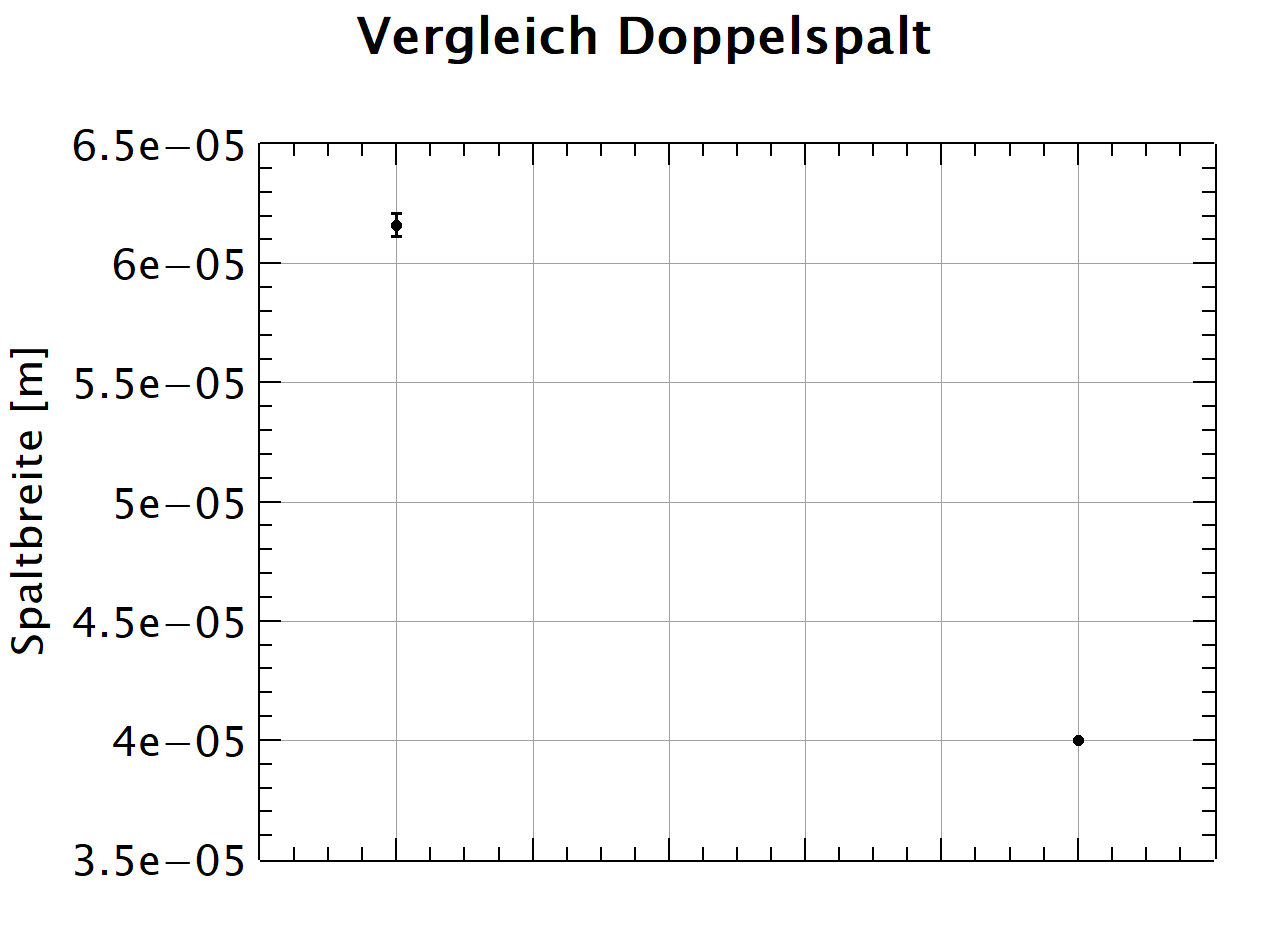
\includegraphics[width=0.4\textwidth]{data/dis_doppel.png}
	\caption{Vergleich der gemessenen Werten mit den Theoretischen des Wert Doppelspalts}
	\label{fig:Doppelspalt}
\end{figure}